\subsection{\dots entropy \dots}

\dots

The learning problem was introduced in \cite{TheorRobopsy} where the main idea was to learn the transition rules of an unknown Turing machines from its known consecutive configurations.

\dots

If we use finite $configN$ configurations then the uncertainty of determining the applied rule between two consecutive configurations can appear during the operation of the learning machine $S$. This uncertainty can be considered as the entropy of the learning machine that can be eliminated easily by the configN++ based universal leraning machine shown in Fig. \ref{fig_ULM}.

\cite{Turing}
\cite{Neumann}
\cite{TheorRobopsy}
\cite{WhatIsLife}

\begin{figure}[!h]
\centering
\scalebox{1}{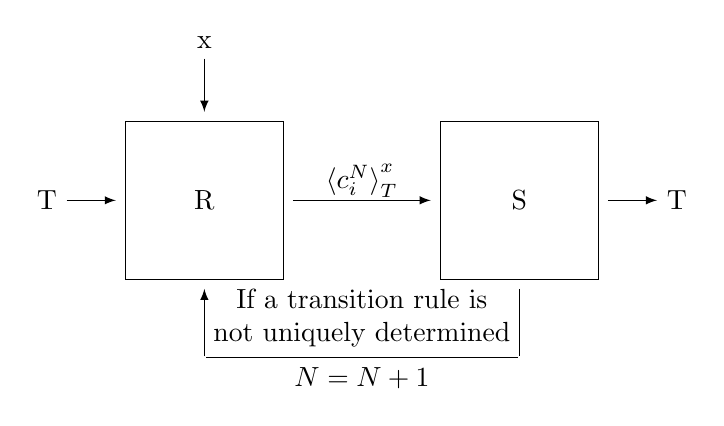
\begin{tikzpicture}

\draw  (-4,3.5) rectangle (-2,1.5);
\draw  (0,3.5) rectangle (2,1.5);
\node (v2) at (-5,2.5) {T};
\node (v1) at (-4,2.5) {};
\node (v4) at (-2,2.5) {};
\node (v3) at (0,2.5) {};
\node (v6) at (2,2.5) {};
\node (v5) at (3,2.5) {T};
\draw [-latex] (v2) edge (v1);
\draw [-latex] (v4) edge (v3);
\draw [-latex] (v6) edge (v5);
\node (v7) at (-3,3.5) {};
\node (v8) at (-3,4.5) {x};
\draw [-latex] (v8) edge (v7);
\node at (-3,2.5) {R};
\node at (1,2.5) {S};
\node at (-1,2.75) {${\langle c_i^N\rangle}_T^x$};
\node at (3,2.5) {};
\node  (v9) at (1,1.5) {};
\node [inner sep=0,outer sep=0](v10) at (1,0.5) {};
\node [inner sep=0,outer sep=0](v11) at (-3,0.5) {};
\node (v12)at (-3,1.5) {};

\draw (v9) edge (v10);
\draw (v10) edge (v11);
\draw  [-latex] (v11) edge (v12);

\node[align=center, below] at (-1,1.5) {If a transition rule is\\not uniquely determined};

\node[below] at (-1,0.5) {$N = N + 1$};
\end{tikzpicture}}
\caption{This figure shows the architecture of a universal learning machine called configN++ based universal leraning machine. The operation of the machine $S$ is based on the Lemma 3.2.1 of \cite{TheorRobopsy}. $R$ uses $configN$ configurations that is denoted by the parameter $N$ in the sequence of configurations ${\langle c^N_i\rangle}_T^x$. If a transition rule is not uniquely determined then $S$ halts and $R$ restarts the simulation of $T$ by using a larger size of configuration.\label{fig_ULM}}
\end{figure}
